\chapter{Souborové systémy OS Linux}
%\todo{Srovnani ext3, ext4, udf, fat, ntfs, ... a nastroju pro ně, soustředit se na fsck}
%\todo{Vysvětlit co to je souborový systém?}

\section{Fyzická úložná média}
%\todo{Ozdrojovat...}
Fyzická úložná média představují nejnižší vrstvu  a zároveň základní kámen všech souborových systémů, protože právě na základě jejich vlastností byly vytvářeny.\\
Z historického hlediska po současnost vývoj přešel přes několik technologií počínaje děrnou páskou a děrnými štítky přes magnetické ukládáním informace do různých nosných médií, optická média po flash paměti. Z hlediska souborových systémů má smysl mluvit až o magnetických médiích, která byla použita pro běžnou práci, protože například lineární pásková úložiště nebyly konstruovány pro kompatibilitu s ostatními systémy ale pouze pro vlastní potřeby, tudíž záznam neobsahoval metadata ale pouze data samotná a jejjich struktura byla uložena jinde nebo vůbec. První opravdové použití souborového systému přišlo až s nástupem disket a pevných disků. \\
První opravdový souborový systém v Unixu byl \textbf{S5FS} neboli \emph{System V File System} (1974), často ovšem označovaný pouze jako \textbf{FS} (File System) nebo \textbf{UFS} (Unix File System) který byl implementován v \emph{UNIX System V} běžící například na mainframech PDP-11. Tento souborový systém byl velice pomalý a také poměrně jednoduchý, ale právě jeho architektura posloužila jako vzor většiny následujících unixových souborových systémů. Tomu ovšem předcházel souborový systém pro mikropočítače s názvem \textbf{CP/M} (1973) neboli \emph{Control Program/Monitor} a později \emph{Control Program for Microcomputer}. Tento souborový systém byl určen narozdíl od S5FS pro mikropočítače od společnosti Intel. V době vzniku totiž začal Intel vyrábět první osmibitové procesory Intel 8008 a o rok později v roce 1974 vznikl Intel 8080 a právě s ním se rozšířil i CP/M. CP/M byl někde na pomezí mezi souborovým a operačním systémem. Na úložném médiu (v tomto případě disketě) byl BIOS, který poskytoval systémová volání na zápis a čtení, řízení klávesnice a monitoru. Poté bylo CP/M, které využívalo těchto volání a poskytovalo je spolu s dalšími shellu a uživatelskému programu. Systémová volání které přidalo CP/M se týkaly převážně přístupu k souborům, která CP/M uchovávalo. Dalším významným souborouvým systémem, který vznikl pro diskety byl \textbf{FAT12} (1977). Posléze s rozšířením pevných disků se začaly vyvíjet další nové souborové systémy odpovídající požadavkům.\\
Z hlediska struktury disku lze mluvit o CHS (Cylinder Head Sector), které rozdělilo úložné médium ve třech rozměrech podle jednotlivých stop (Cylinder), čtecí hlavy (Head), kterých může být u pevných disků více, záleží na počtu jednotlivých disků a použitých stran a poslední rozměr je sektor (Sector), který určuje o kterou část stopy jde. Právě sektory dostály ve vývoji největších změn, protože původní dělení po úhlech od středu disku nebylo efektivní se vzrůstající vzdáleností od středu. Proto se později přešlo k dělení na jednotnou velikost sektoru, které se rozložily rovnoměrně po celém disku.\\
Sektor je nejmenší zápisovou jednotkou na médiu, která je určená výrobcem média. Typicky se jedná o velikosti 512~B u pevných disků, 2048~B u CD-ROM a DVD-ROM. Nové pevné disky používají velikost bloku 4096~B. Důvodem pro členění po sektorech je zjednodušení přístupu k médiu za předpokladu, že uložená data jsou větší než velikost bloku. V opačném případě dochází k plýtvání místem, protože se vždy čte a zapisuje celý blok. Právě proti sektorům se obvykle navrhují bloky souborového systému, které se snaží využít sektory co nejefektivněji jak z hlediska úspory místa tak z hlediska přístupového a zápisového času.

\section{Diskové oddíly}
Diskové oddíly představují způsob, jak lze fyzické médium abstraktně rozdělit na více částí. Rozdělení na oddíly je uloženo v MBR (Master Boot Record) a jeden disk může obsahovat až 4 hlavní oddíly. V případě potřeby více oddílů lze použít rozšířený oddíl, který zapouzdřuije další dělení na oddíly, ovšem tentokrát již mimo MBR.\\
Důvodem pro rozdělení na oddíly může být oddělení uživatelských dat od systémových, vyhrazení místa pro odkládací oddíl nebo jiné logické dělení. 

\section{Logical Volume Manager (LVM)}
%\todo{https://wiki.archlinux.org/index.php/LVM}
Logical Volume Manager (LVM) představuje způsob abstrakce nad diskovými oddíly. Ačkoli se může zdát, že se jedná o podobnou technologii jako je RAID, není tomu tak (\cite{arch-lvm}).\\
LVM vzniklo pro zajištění větší flexibility pro organizaci úložiště. Představte si situaci na následujícím obrázku:
\pagebreak
\begin{verbatim}
Disk1 (/dev/sda):
 _ _ _ _ _ _ _ _ _ _ _ _ _ _ _ _ _ _ _ _ _ _ _ _ _ _ _ _ _ _ _ _ _ _ _ _ _
|Partition1 50GB (Physical volume) |Partition2 80GB (Physical volume)     |
|/dev/sda1                         |/dev/sda2                             |
|_ _ _ _ _ _ _ _ _ _ _ _ _ _ _ _ _ |_ _ _ _ _ _ _ _ _ _ _ _ _ _ _ _ _ _ _ |
                                                     
Disk2 (/dev/sdb):
 _ _ _ _ _ _ _ _ _ _ _ _ _ _ _ _ _ _ _ _ _ _ _ _ _ _
|Partition1 120GB (Physical volume)                 |
|/dev/sdb1                                          |
| _ _ _ _ _ _ _ _ _ _ _ _ _ _ _ _ _ _ _ _ _ _ __ _ _|
\end{verbatim}
Jak je vidět, situace obsahuje dva disky, každý o jiné velikosti a formátu. Pokud bychom chtěli vytvořit diskový oddíl, museli bychom sáhnout po řešení RAID 0 a disky posléze naformátovat dle potřeby. V případě změny velikosti by bylo nutné uložiště přeformátovávat. Ovšem při použití LVM situace vypadá například takto:
\begin{verbatim}
Volume Group1 (/dev/MyStorage/ = /dev/sda1 + /dev/sda2 + /dev/sdb1):
 _ _ _ _ _ _ _ _ _ _ _ _ _ _ _ _ _ _ _ _ _ _ _ _ _ _ _ _ _ _ _ _ _ _ _ _ _ 
|Logical volume1 15GB  |Logical volume2 35GB    |Logical volume3 200GB    |
|/dev/MyStorage/rootvol|/dev/MyStorage/homevol  |/dev/MyStorage/mediavol  |
|_ _ _ _ _ _ _ _ _ _ _ |_ _ _ _ _ _ _ _ _ _ _ _ |_ _ _ _ _ _ _ _ _ _ _ _ _|
\end{verbatim}
Všechny oddíly byly sloučeny do jedné logické skupny s názvem \texttt{MyStorage} s velikostí 250~GB a to bylo následně pouze logicky rozděleno na oddíly jak je vidět na obrázku. Tyto logické oddíly posléze budou naformátovány libovolným souborovým systémem.\\
Zásadní rozdíl oproti RAID 0 je v možnostech změny struktury úložiště. V případě RAID 0 se změna promítá do formátování RAID úložiště, v případě LVM se jedná o změnu velikosti logické jednotky pouze za předpokladu existence nějakého volného místa, nezávisle na jeho místě na disku. Tudíž není třeba přesouvat oddíly pro potřeby jejich zvětšení.

\section{Srovnání souborových systémů}
Pro operační systém Linux bylo během jeho existence vyvinuto mnoho různých souborových systémů stejně tak jako jich bylo mnoho implementováno z ostatních operačních systémů. Některé z nich jsou používány i v současnosti, některé byly opuštěny nebo nahrazeny.\\
Podle \cite{tldp-filesystem} patří mezi nejvýznamnější nativní souborové systémy tyto:
\begin{itemize}
    \item minix -- nejstarší souborový systém OS Linux. Vzhledem k jeho stáří se dnes již aktivně nevyvýjí a nepoužívá. Mezi jeho hlavní omezení patří maximální velikost souborového systému, která je až 64~MB. Dalším významným omezením je délka názvů soborů, která je limitována na 30 znaků.
    \item ext -- tento souborový systém, celým jménem Extended Filesystem, vznikl v roce 1992 speciálně pro potřeby kernelu OS Linux \cite{linmag-ext}. Jeho inspirací byl souborový systém UFS (Unix File System), ze kterého převzal strukturu metadat. Jeho limitací byla maximlní velikost 2~GB.
    \item ext2 -- nástupce souborového systému ext. Byla navýšena maximální velikost na 32~TB a byl navržen podle stejných principů jako Berkeley Fast File System z projektu BSD \cite{nongnu-ext2}. Dlouhou dobu byl tento souborový systém používán ve všech hlavních distribucích OS Linux. ext2 nebyl zpětně kompatibilní s původním ext.
    \item ext3 -- již v pořadí třetí verze ext souborového systému. Nyní již byla zachována téměř plná zpětná kompatibilita s ext2. Oproti ext2 ovšem ext3 přineslo žurnálování, které pomohlo v obnově souborového systému při chybě systému \cite{paper-ext3}. Zbytek parametrů zůstal shodný s ext2.
    \item ext4 -- současná verze ext souborového systému \cite{paper-ext4}. Opět je zpětně kompatibilní s ext3 a ext2 ale oproti nim byla navýšena maximální velikost na 1~EB, ale doporučené maximum je 16~TB. Původně byl ext4 pouze skupina rozšížení pro ext3, ale později se osamostatnil jako ext4. Dalším rozšířením je nyní již neomezený počet podsložek (ext3 mělo omezení na 32000 podsložek). Také bylo zlepšena odolnost žurnálu přidáním kontrolních součtů a celková výkonnost souborového systému.
    \item vfat -- typický zástupce cizích souborových systémů. V tomto případě se jedná o MS FAT32, který je hojně používaný na USB flash discích.
    \item iso9660 -- standardní souborový systém pro CD-ROM. 
    \item udf -- souborový systém původně vyvynutý pro datové rozšíření CD-ROM. Posléze rozšířen pro DVD a BluRay. V současnosti je používán například v šifrovaných flash discích. 
    \item smbfs -- síťový souborový systém Samba File Systém vyvynutý pro sdílení dat mezi počítači s MS Windows. Podporuje Windows Sharing Protocol.
    \item ntfs -- v současnosti nejpoužívanější souborový systém v MS Windows.
\end{itemize}

\section{Nástroje kontroly integrity}
V prostředí OS Linux je pro kontrolu integrity určen primárně nástroj \texttt{fsck} (Filesystem Consistency Check). V manuálové stránce k \texttt{fsck} \cite{man-fsck} se lze dočíst, že samotný \texttt{fsck} je pouze frontend, který volá specifické nástroje pro daný souborový systém. Skutečné nástroje určené pro kontrolu integrity, které jsou obvykle dodávány spolu s nástroji k vytvoření a práci s daným soborovým systémem se jmenují \texttt{fsck.fstype}, například \texttt{fsck.ext4}.\\
Pro masivně používané souborové systémy tyto nástroje existují. Pro \textbf{ext} rodinu se jedná o nástroj \texttt{e2fsck}. Podporovány jsou i převzaté souborové systémy, například \texttt{fsck.fat} pro souborové systémy \textbf{vfat} a \textbf{msdos}. Ovšem pro například pro \textbf{iso9660} nástroje kontrolující integritu existují pouze jako nástroje vzniklé na základě pokusů při testování vadných disků. Takovým je i \texttt{isovfy} \cite{man-isovfy} ze skupiny nástrojů isoinfo, který ovšem pouze umožňuje kontrolu integrity, nikoli opravu chyb.\\
Nástrojem který v tuto chvíli chybí je podle všeho \texttt{fsck.udf}. Projekt ve s názvem udftools \cite{udftools-sourceforge} ve kterém vznikl i podprojekt udffsck byl autorem opuštěn v roce 2004 a nástroj pro kontrolu konzistence nebyl nikdy započat. 

\chapter{Universal Disk Filesystem}
\label{sec:udf}
%\todo{Popsat filesystem, způsob uložení dat, ochrané mechanismy... UDF docs rulez!}
Universal Disk Filesystem (UDF) je souborový systém navržený pro použití na CD, DVD a Blu-Ray discích ale díky jeho univerzálnosti je možné jej použít i na jiných médiích. Jeho návrh vyšel ze systému CDFS (ISO 9660) ale není s ním kompatibilní. Jednou z výhod UDF oproti CDFS je například možnost dodatečného zápisu na CD anebo naopak mazání dat z CD. 

\section{Struktura systému}
Norma popisující UDF popisuje dva druhy číslování. Prvním je \textit{Logical Sector Number} (LSN), které popisuje čísla jednotlivých sektorů. Je číslované od nuly a začíná na prvním fyzickém sektoru média. Jeho velikost by měla odpovídat fyzické velikosti sektoru. Jeho určením je fyzická navigace na médiu. Druhým je \textit{Logical Block Number} (LBN), které popisuje čísla jednotlivých logických bloků, které jsou mapovány na sektory. Jejich velikost by měla být stejná jako je velikost sektorů. Jsou číslované od nuly ale začínají až v oblasti dat. Jeho určením je na rozdíl od LSN navigace pouze v datech.\\
Samotné médium je rozděleno do pěti částí. První je \textit{Volume Recognition Sequence} (VRS). Tato část je lokalizována na fixní adrese \texttt{0x10000}, což odpovídá sektoru 16 při velikosti sektoru 2~kB. Důvodem této fixní adresy je právě dodržení zpětné kompatibility se standardem ISO9660, který předpokládá použití pouze na optických médiích s velikostí sektoru 2~kB. Tato zpětná kompatiblita pokračuje dále v tom smyslu, že celá VRS je dále zpracovávána právě po 2~kB blocích, pokud je velikost fyzického sektoru menší nebo stejná. V opačném případě je nutné přejít k blokům větším a zpětná kompatibilita je porušena. Význam VRS je identifikace použitého souborového systému na médiu. Více o VRS je v samostané kapitole \ref{sec:vrs}.\\
Další částí je \textit{Anchor Volume Descriptor Pointer} (AVDP). Tato část je již pouze pro UDF a jedná se o výchozí bod při čtení souborového systému. Mají několik různých umístění a typicky je na médiu víckrát. Obsahuje jedinou informaci a tou je umístění \textit{Volume Descriptor Sequence} (VDS) a to jak hlavní, tak záložní. Více je v kapitole \ref{sec:avdp}.\\
Následující částí je již zmíněný \textit{Volume Descriptor Sequence} (VDS). Tato skupina deskriptorů popisuje veškeré vlastnosti souborového systému, jeho stav a další. Je zaznamenána vždy ve dvou exemplářích pro zvýšení robustnosti. VDS je detailněji popsána v kapitole \ref{sec:vds}.\\
Další částí je \textit{Logical Volume Integrity Descriptor} (LVID), který popisuje integritu souborového systému. Více je v kapitole \ref{sec:lvid}. Tímto deskriptorem končí metadata systému.\\
Poslední částí jsou samotná data. Jejich výchozím bodem je \textit{File Set Descriptor} (FSD), který udržuje informaci o počtu adresářů a souborů a umístění kořenového adresáře. Poté následují už samotné deskriptory dat následované daty.\\
Vzhledem k možné koexistenici s ISO9660 na médiu je možné že budou existovat i struktury tohoto souborového systému. Tuto skutečnost je potřeba mít na paměti při případném zápisu dat na médium. Pro samotné čtení není třeba se nad tímto déle pozastavovat.

\section{Deskriptory UDF systému}
Tato část stručně popisuje skupiny deskriptorů souborového systému UDF. Jedná se pouze o přehledovou část vzhledem k velkému překryvu s specifikací, která je uvedena v \cite{osta-udf-0201} a standardem ECMA-167, který je uveden v \cite{ecma-167}.

\subsection{UDF Bridge Volume Recogniton Sequence}
\label{sec:vrs}
Tato sekce je určena k rozpoznání obsaženého souborového systému. Jak bylo předesláno v předchozí kapitole, může být velká až 6 sektorů a obsahuje deskriptor identifikující souborový systém. Jeho poloha je fixní na sektoru 16.\\
Struktura deskriptorů je zachycena v tabulce \ref{tab:vrs}.
\begin{table}
    \begin{tabular}{ | l | l | l | l | l | }
        \hline
        Adresa  & Délka [B]   & Jméno položky & Datový typ    & Popis \\ \hline
        0       & 1             & Type           & int8          & Typ deskriptoru \\ \hline
        1       & 5             & Identifier & string        & Identifikátor typu souborového systému \\ \hline
        6       & 1             & Version         & int8          & Verze deskriptoru \\ \hline
        7       & 2041          & ---           & ---           & Volné místo, záleží na typu deskriptoru \\ \hline
    \end{tabular}
    \caption{Struktura VRS deskriptorů\label{tab:vrs}}
\end{table}
Jak je vidět, deskriptor se skládá ze třech částí, pomineme-li poslední rezervovanou část obsahující volné místo. První položka \textit{Type} určuje typ deskriptoru. V tomto případě je jediná povolená hodnota 1. Další položka s názvem \textit{Identifier} obsahuje řetězec o pěti znacích. Tato část určuje typ použitého souborového systému. Možné varianty jsou tyto:
\begin{itemize}
    \item \texttt{BOOT0} - Bootovací záznam
    \item \texttt{CD001} - Souborový systém ISO~9660
    \item \texttt{CDW02} - Souborový systém podle ECMA-168
    \item \texttt{BEA01} - \textit{Beginning Extended Area Descriptor}, začátek UDF Bridge sekvence
    \item \texttt{TEA01} - \textit{Terminating Extended Area Descriptor}, konec UDF Bridge sekvence
    \item \texttt{NSR01} - UDF verze 1.0 a vyšší
    \item \texttt{NSR02} - UDF verze 1.5 a vyšší
    \item \texttt{NSR03} - UDF verze 2.0 a vyšší
\end{itemize}
Poslední položkou je \textit{Version} která obsahuje inforamci o verzi deskriptoru. Zde by měla být v těchto případech vždy \texttt{0x01}.\\
Aby mohlo být prohlášeno, že médium obsahuje UDF, musí být nalezen deskriptor obsahující \textit{Identifier} s hodnotou \texttt{NSR01}, \texttt{NSR02} nebo \texttt{NSR03}. V opačném případě se nejedná o UDF.

\subsection{Anchor Volume Descriptor Pointer}
\label{sec:avdp}
\textit{Anchor Volume Descriptor Pointer} (AVDP) je klíčová část souborového systému. Tato struktura udržuje adresu deskriptorů souborového systému a jejich délku. Právě AVDP je první deskriptor, který se čte po identifikaci souborového systému, proto je umístěn na předem známém místě. V případě uzavřených souborových systémů to je na sektoru 256, posledním sektoru média a nezřídka také na 256 sektoru od konce média. V případě otevřených souborových systémů je zde výjimka, protože AVDP je na dočasně umístěno na sektoru 512 až do uzavření systému.\\
Jeho struktura je vidět na tabulce \ref{tab-avdp}. Jak je vidět, obsahuje ukazatele na hlavní a záložní VDS což zvyšuje robustnost celého souborového systému.
\begin{table}[hb]
    \begin{tabular}{ | l | l | p{4.5cm} | p{1.3cm} | p{5.5cm} | }
        \hline
        Adresa  & Délka [B]   & Jméno položky & Datový typ    & Popis \\ \hline
        0       & 16          & DescriptorTag & struct        & Popis deskriptoru \\ \hline
        16      & 8           & MainVolumeDescriptor SequenceExtent & struct & Sektor a délka \textit{Main Volume Descriptor Sequence} \\ \hline
        24      & 8           & ReserveVolumeDescriptor SequenceExtent & struct & Sektor a délka \textit{Reserve Volume Descriptor Sequence} \\ \hline
        32      & 480         & Rezerva & & \\ \hline
    \end{tabular}
    \caption{Anchor Volume Descriptor Pointer\label{tab-avdp}}
\end{table}

\subsection{Volume Descriptor Sequence}
\label{sec:vds}
\textit{Volume Descriptor Sequence} (VDS) je skupina deskriptorů popisující veškeré vlastnosti souborového systému UDF. Jsou seřazeny postupně na jednotlivých sektorech počínaje adresou udanou z AVDP \ref{sec:avdp} a končí po počtu uloženém opět v AVDP. Jsou uloženy postupně po sektorech od výchozí adresy a končí \textit{Terminating Descriptor}, což je prázdný deskriptor, který obsahuje pouze \textit{Descriptor Tag}. Samotné pořadí deskriptorů není pevné a samotné deskriptory jsou identifikovány právě pomocí \textit{Descriptor Tag}.\\
Jak je vidět v AVDP, i tato část je uložena duplicitně pro zvýšení robustnosti. Rezervní VDS je uložena ve stejném tvaru jako primární tentorkát však od jiné adresy, opět uvedené v AVDP.\\
Samotné deskriptory jsou popsány v \cite{osta-udf-0201}, kapitola 2.2. Pro kompletnost zde uvedu jejich výčet ze standardu verze 2.01.
\begin{itemize}
    \item \textit{Primary Volume Descriptor}
    \item \textit{Logical Volume Descriptor}
    \item \textit{Unallocated Space Descriptor}
    \item \textit{Implementation Use Volume Descriptor}
    \item \textit{Partition Descriptor}
    \item \textit{Terminating Descriptor}
\end{itemize}

\subsection{Logical Volume Integrity Sequence}
\label{sec:lvid}
Další důležitou částí je \textit{Logical Volume Integrity Descriptor} (LVID) spolu s \textit{Terminating Descriptor} (TE). Tato sekvence je uložena pouze jednou a její umístění je udržováno v LVD. Obsahuje následující informace:
\begin{enumerate}
    \item Je Logický svazek v konzistentním stavu?
    \item Kdy bylo naposledy cokoli na Logickém svazku modifikováno.
    \item Kolik bloků je volných na svazku?
    \item Jaká je celková velikost svazku v blocích?
    \item Byl obsah modifikován nějakou \textit{jinou} implementací od posledního přístupu implementace která svazek vytvořila?
\end{enumerate}
Jak je vidět z tohoto výčtu, tato část je důležitá hlavně pro čtení a zápis, ale i pro kontrolu dat má svůj význam, například právě kvůli informaci o konzistenci svazku.\\ 
Samotný formát struktury je opět v \cite{osta-udf-0201}, kapitola 2.2.6.

\section{File Structure}
\label{sec:fsd}
Souborová struktura UDF je postavena na třech deskriptorech, které se podílí na popisu a uložení dat. Jedná se o tyto deskriptory:
\begin{itemize}
    \item \textit{File Set Descriptor} (FSD)
    \item \textit{File Entry} (FE)
    \item \textit{File Identifier Descriptor} (FID)
\end{itemize}

\subsection{File Set Descriptor}
\label{sec:fsd}
\textit{File Set Descriptor} (FSD) je výchozím bodem pro čtení dat. Jeho pozice je opět uložena v LVD. Jeho struktura je popsána v \cite{osta-udf-0201}, kapitola 2.3.2. Tato strukutra mimo jiné obsahuje umístění kořenového adresáře. Z hlediska kontroly dat nejsou ostatní údaje tolik významné.

\subsection{File Entry}
\label{sec:fe}
\textit{File Entry} (FE) je deskriptor, který popisuje samotný soubor. Jeho pozice je určena jeho \textit{rodičem}, což v případě kořenového adresáře je FSD, ale uvedený je opět kořenový adresář, v případě ostatních souborů a adresářů se jedná o adresář, v němž se nachází.\\
Jeho struktura je popsána v \cite{osta-udf-0201}, kapitola 2.3.6, a z ní pouze vyberu některé důležité části. První důležitou informací je počet zapsaných bloků (\textit{LogicalBlocksRecorded}). Další důležitou částí jsou \textit{AllocationDescriptors}. Velikost této části je určena pomocí \textit{LengthofAllocationDescriptors} a obsahuje dva druhy dat, podle toho jestli se FE popisuje adresář nebo soubor.\\
V případě souboru je v tomto místě uložena pozice dat souboru ve formě \textit{Long Allocation Descriptor} nebo \textit{Short Allocation Descriptor}. Vždy bude použit pouze jeden z nich a měl by být uložen pouze jeden, protože data jsou ukládána sekvenčně do bloků za sebou.\\
V případě adresáře jsou v \textit{AllocationDescriptors} uloženy \textit{File Identifier Descriptor} (kapitola \ref{sec:fid}), přičemž každý jeden deskriptor drží informaci o jednom \textit{potomkovi} adresáře. Vždy je přítomen nejméně jeden FID a tím je \textit{rodičovský adresář}. 

\subsection{File Identifier Descriptor}
\label{sec:fid}
\textit{File Identifier Descriptor} (FID) je struktura, která udržuje informace o souboru na úrovni mateřského adresáře. Je popsaný v \cite{osta-udf-0201} v kapitole 2.3.4.\\
Vzhledem k faktu, že cílem této struktury není adresovat data ale jen FE, obsahuje jen metadata metadat souboru. Například jestli adresované FE popisuje složku nebo soubor, jestli je soubor smazaný nebo jestli uživatel má vědět o existenci souboru. Dále tato struktura obsahuje identifikátor souboru v podobě textového řetězce (jméno souboru nebo složky). Samozřejmě obsahuje i umístění samotného FE.


\chapter{Definice chyb na souborovém systému}
%\todo{Jak se to může pokazit? A co se s tím dá dělat?}
Chyby na souborovém systému mohou vzniknout ze třech příčin. 
\begin{enumerate}
    \item Chybou ovladače souborového systému,
    \item nekorektním odpojením souborového systému (například odpojení flash disku před ukončením všech transakcí),
    \item fyzickým poškozením média (například stářím poškozené bloky flash paměti nebo poškrábané optické médium).
\end{enumerate}
První druh chyb se děje zřídka. Důvodem je skutečnost, že programy a kernelové moduly starající se o přístup k a práci se souborovými systémy bývají dobře odladěné a otestované. Koneckonců, právě data jsou to, co má v počítačích hodnotu.\\
Druhý druh chyb se vyskytuje velice často. Odebrání disku ve spěchu bez korektního odpojení může způsobit poškození souborového systému skrz přerušení probíhající zápisové operace. Systém poté zůstane v nekonzistentním stavu, protože se tam nachází částečně zapsaný soubor. Případně může dojít k poškození metadat souboru. Do této kateogie spadají i chyby vzniklé havárií operačního systému.\\
Třetí kategorií chyb jsou veškeré poruchy fyzického média. U optických disků se první vybaví škrábance a rýhy. Tyto chyby poté bývají shluknuty do clusterů poškozených dat. U magnetických disků může dojít k poškození kolizí čtecích hlav s plotnou nebo k poškozením opotřebením. V dnešní době se dá předejít obojímu. Vyšší řady disků určených pro notebooky mají integrovaný akcelerometr a v případě většího zrychlení dojde k nouzovému zaparkování čtecích hlav. Chybám z opotřebení lze předcházet pomocí integrovaného systému S.M.A.R.T. který se stará o sběr telemetrických dat o disku a na jejich základě lze předvídat jeho poruchu. S příchodem FLASH technologie se objevil druh chyb ve formě vadných paměťových buněk, ať už z výroby nebo opotřebením. V jistém malém procentu případů (které významně roste s nadmořskou výškou až nabývá kritické významnosti například u palubních systémů v letectví) může dojít i k vytvoření chyby pomocí vysoce nabité částice, která změní napěťový potenciál v bitu.\\
Opravitelnost a analýza chyb je vždy otázkou míry a typu poškození.

\section{Detekce chyb}
\label{sec:errordetection}
Způsobů jak detekovat chyby v případě jejich nastání je celá řada a liší se požadavky na prostředky a čas. Za naivní přístup lze považovat například detekci porovnáním s referencí. Předpokládejme, že máme stejnou informaci uloženou dvakrát na různých místech (médiích) a v případě poruchy dat je možné data obnovit z referenčního média. Tento přístup představuje například RAID nebo také diferenciální vedení. Toto řešení je evidentně náročné na úložiště kvůli stoprocentní duplicitě dat. Výměnou za to poskytuje informaci nejen o přítomnosti chyby ale i o její poloze a původních datech. Dalším přístupem je vytváření kontrolních součtů. Tento přístup nám dává oproti předchozímu pouze informaci o přítomnosti chyby bez informace kde chyba je a jak ji opravit. V absurdním případě se můžou chyby dokonce navzájem vyrušit takže data nebudou konzistentní ale kontrolní součet bude stejný. I přes tyto nedostatky je kontrolní součet oblíbená metoda detekce chyb kvůli své jednoduchosti a nenáročnosti na paměť. Poněkud komplexnější variantou je CRC (Cyclic Redundancy Check). Tento mechanismus, který původně vznikl pro kabelové přenosy našel uplatnění všude, kde je potřeba mít možnost chyby nejen detekovat ale i opravovat a přitom není prostor pro kopii dat. Je výpočetně náročnější ale výsledek je opět několikabytové číslo. I zde může v extrémním případě dojít k poškození dat a nezměnění CRC, ale tato šance je řádově nižší než v případě kontrolního součtu.

\subsection{Cyclic Redundancy Check}
\label{sec:crc}
Cyclic Redundancy Check je narozdíl od ostatních metod poněkud složitější a proto si zaslouží vysvětlení. CRC se skládá z několika částí. Výchozí částí je generační polynom (GP), který určuje na jaké chyby bude naše CRC citlivé. Generační polynom je vytvořen jako sekvence jedniček a nul o stejné délce jako výsledné CRC. Pro polynom $GP=1 \cdot x^3 + 0 \cdot x^2 + 1 \cdot x^1 + 0 \cdot x^0$ odpovídá podle koeficientů GP 1010.\\
Výchozí operací která je jádrem CRC je logická funkce XOR. Pro demonstraci výpočtu CRC si nadefinujeme řetězec dat, pro která je potřeba CRC spočítat.
\begin{verbatim}
Data: 0100 1011 0001 1111 1100
\end{verbatim}
K těmto datům je potřeba připojit tolik nul, kolik má být délka výsledného CRC, takže výsledek vypadá následovně.
\begin{verbatim}
Data: 0100 1011 0001 1111 1100 0000
                               ----
\end{verbatim}
Nyní je potřeba spočítat samotné CRC. To se provádí postupným XORem nad daty a posléze mezivýsledky tak dlouho, dokud nedojdeme s generačním polynomem až na konec dat. Důležitá poznámka je, že generační polynom se vždy zarovnává s nejbližší jedničkou a až poté probíhá XOR. Poté to co zbylo je naše CRC a to se přidá k datům do vyhrazené oblasti, kterou jsme přidali v předchozím kroku.
\begin{verbatim}
     0100 1011 0001 1111 1100 0000
XOR   101 0
1.   -----------------------------
     0001 1011 0001 1111 1100 0000
XOR     1 010
2.   -----------------------------
     0000 1111 0001 1111 1100 0000
XOR       1010
3.   -----------------------------
     0000 0101 0001 1111 1100 0000
XOR        101 0
4.   -----------------------------
     0000 0000 0001 1111 1100 0000
XOR               1 010
5.   -----------------------------
     0000 0000 0000 1011 1100 0000
XOR                 1010 
6.   -----------------------------
     0000 0000 0000 0001 1100 0000
XOR                    1 010
7.   -----------------------------
     0000 0000 0000 0000 1000 0000
XOR                      1010
8.   -----------------------------
     0000 0000 0000 0000 0010 0000
XOR                        10 10
9.   -----------------------------
     0000 0000 0000 0000 0000 1000
                              ----
\end{verbatim}
Na tomto příkladu jsme demonstrovali výpočet 4-bitového CRC nad 20 bity dat. Výsledné CRC je 1000.\\
Detekce chyby může být provedena dvěma způsoby. Buď stejně jako u kontrolního součtu prostým výpočtem CRC nad daty bez vlastního CRC a jejich porovnáním anebo hledáním chyby pomocí chybového vektoru. V případě, že jsou data správná, po operaci XOR nad celými daty včetně CRC musí vyjít chybový vektor 0. Ovšem pokud je datech chyba, vektor vyjde nenulový.

\section{Použité kontrolní mechanismy v UDF}
\label{sec:howtolabelthat}
V UDF se využívá několika různých mechanismů, které jsou i v případě nutnosti kombinovány pro zvýšení robustnosti.
\begin{itemize}
    \item Redundace dat na médiu,
    \item zápisový bit,
    \item checksum,
    \item CRC.
\end{itemize}
V tomto výčtu jsou zachyceny všechny kontrolní mechanismy na úrovni UDF. Kontrolní součty jsou popsány v kapitolách \ref{sec:errordetection} a \ref{sec:crc}. Konkrétně je checksum použit pro kontrolu \textit{DescriptorTag} a CRC pro kontrolu samotného deskriptoru, přičemž jeho referenční výsledek je uložený v již zkotrolovaném tagu.\\
Redundace deskriptorů byla zmíněna v kapitole \ref{sec:udf}. Lze si povšimnout, že čím je deskriptor důležitější pro samotnou funkci souborového systému, tím je jeho fyzická vzdálenost mezi jednotlivými výskyty na médiu větší. V případě AVDP, které je klíčové pro funkci je jeho vzdálenost téměř maximální možná vzhledem k velikosti média (poprvé je uložen na sektoru 256 a poté na konci média). Další případ redundance je v případě VDS.\\
Zápisový bit je aplikační ošetření konzistence dat. Jeho fuknci lze přirovnat k zámku na vypínači. Pokud je bit nastaven do logické nuly, zápis probíhá (anebo spíše byl přerušen a nebyl korektně ukončen) zatímco pokud pokud je v logické jedničce, tak to značí korektně ukončenou zápisovou operaci.

\chapter{Realizace nástroje pro detekci chyb}
%\todo{Vlastní řešení.}
%\todo{https://github.com/illumos/illumos-gate/tree/master/usr/src/cmd/fs.d/udfs/fsck}
\section{Stav projektu udftools}
Projekt udftools byl založen roce 1999 na projektovém serveru SourceForge \cite{udftools-sourceforge} Bennem Fennemou. Byl implementován standard UDF 1.5 a byly vytvořeny nástroje pro paketový zápis na CD, vytvoření souborového systému UDF a pro přístup k němu. Nástroj pro kontrolu konzistence zůstal jako prázdný projekt, byly ovšem vytvořeny nástroje pro vytvoření souborového systému UDF, nástroje pro jeho zápis včetně paketového zápisu.\\
V roce 2007 byly integrovány poslední patche a poté projekt zůstal ležet ladem. V roce 2014 byl projekt přemigrován na GitHub \cite{udftools-github} Palim Rohárem a znovu byl započat vývoj, převážně opravy starých chyb. Byla implementována verze UDF 2.01. Nástroj \texttt{fsck.udf} nebyl v tomto projektu nikdy vytvořen a tento stav přetrvává do současnosti.\\
V tuto chvíli se komunita okolo projektu udftools skládá hlavně z Paliho Rohára a z Františka Kluknavského. Vzhledem k nepříliš vysoké popularitě UDF není projekt udftools aktivní. Sice je stále udržován panem Rohárem, ale aktivní vývoj v tuto chvíli pravděpodobně neprobíhá, nebo alespoň ne veřejně.

\section{Existující nástroje pro kontrolu konzistence UDF}
Pro OS Linux jsou znám pouze nástroj \texttt{udfct\_1.5r4}. Tento nástroj byl vyvynut firmou Philips a jedná se o nástroj který je schopný zkontrolovat integritu souborového systému UDF. Chyby v implementaci UDF a případné chyby v datech vypisuje do terminálu ale není schopný je opravovat. Zásadním problémem tohoto nástroje je, že existuje pouze pod restriktivní licencí firmy Philips a není jej tudíž možné použít jako výchozí bod dalšího vývoje i přes dostupnost zdrojových souborů. V současnosti je balíček se zdrojovými kódy dostupný na Wayback Machine \cite{wayback}, firma Philips jej již nenabízí. Mou žádost o poskytnutí práva na přepoužití jejich kódu ignorovali.\\
V BSD je \texttt{fsck} v podobném stavu jako v Linuxu ovšem komunita okolo BSD na problému pomalu pracuje. Našel jsem blog \cite{scottuvblog} od Scotta Longa z projektu FreeBSD kde má shrnutí své práce na UDF včetně jeho patchů do FreeBSD implementace UDF. Mezi jeho body k doplnění je i nástroj \texttt{fsck} a právě proto jsem ho oslovil s prosbou o informace. Právě Scott Long mne odkázal na projekt NetBSD, protože on sám nikdy na \texttt{fsck} nezačal pracovat, ale doslechl se, že v projektu NetBSD něco vzniká. Po hledání jsem nalezl mailing list z roku 2008, kde Reinoud Zandijk popisuje svůj postup práce na UDF implementaci. Na konci jeho zprávy je poznámka o \texttt{fsck} s informací, že bude "brzy". Žádná implementace se ovšem na svět nedostala, takže jsem mu napsal s prosbou o informace o  stavu jeho implementace \texttt{fsck}. Jeho odpověď byla vyčerpávající a potvrzovala mé podezření o stavu open source implementace. On sám má rozpracovanou implementaci \texttt{fsck} ale zveřejňovat ji zatím nebude, protože není dokončena, jeho slovy: 
\begin{quote} 
I've created two UDF implementations: UDFclient \cite{13monkey} and the NetBSD UDF implementation. UDFclient was a kind of study into UDF and far too elaborate to be useful for my FSCK implementation, it'll need to be pruned first.
\end{quote} 
Nikdo další žádnou jinou open source implementaci nemá vyjma projektu Open Solaris, což bylo panem Reinoudem Zandijkem okomentováno takto:
\begin{quote}
As for \texttt{fsck\_udf}, there is only one opensource version and thats the OpenSolaris one. Before you get too excited, its fairly limited and will only check older media and even then only deals with recovering free space and get the directory tree in-order. Important but limited.
\end{quote}
Implementace v projektu Open Solaris je tedy v současnosti jedinou dostupnou open source implementací \texttt{fsck}. Jejich kód je dostupný na serveru GitHub \cite{solaris-github}. Bohužel ani jejich implementace není kompletní a dokáže obnovit pouze volné místo a strom souborového systému ale bez dat. Dalším omezením je maximální verze UDF, která je omezena na verzi 2.01 ovladačem UDF. Nástroj jako takový exaktní omezení verze nemá. Ovšem i toto je dobrý výchozí bod pro další práci.\\
Co se týká OSX od společnosti Apple, ti mají nástroje pro kontrolu UDF implementovanou v nástroji \texttt{fsck\_udf} pro všechny exitující revize, ovšem zdrojové kódy nejsou veřejně dostupné, takže je možné jejich nástroje použít pouze jako referenční pro srovnání funkčnosti.\\
Microsoft Windows má implementovaný checkdisk pro UDF ale jeho zdrojový kód je bohužel uzavřený.\\

\section{Implementace nástroje \texttt{udffsck}}
Nástroj \texttt{udffsck} z balíčku \texttt{udftools} navazuje na ostatní nástroje v balíčku, využívá sdílené hlavičky s definicemi UDF a jeho cílem je být plnohodnotným \texttt{fsck} nástrojem pro UDF.\\
Implementace samotná je rozdělena do dvou fází. V první fázi je cílem vytvořit nástroj pro detekci chyb. Jeho cílem není ani obnovovat data ani opravovat chyby v metadatech, ale pouze říct kde je jaká část poškozená, čili víceméně to, co umí nástroj z distribuce Open Solaris. Ve druhé fázi je cílem nalezené chyby opravit, pokud to bude možné. Vzhledem k poměrně vysoké robustnosti samotného UDF díky jeho návrhu pro optická média, kde se předpokládá poškození nosiče, je relativně vysoká šance na úspěch co se týká opravování chyb v metadatech. Samotná data podle všeho opravit nepůjdou.\\
Závěrem implementace je začlenění výsledného \texttt{udffsck} zpět do balíčku \texttt{udftools}, ze kterého je rozvětven.\\
Myšlenkovou strukuturu programu zachycuje obrázek \ref{fig:steps1}. 
\begin{figure}[ht] 
    \centering
    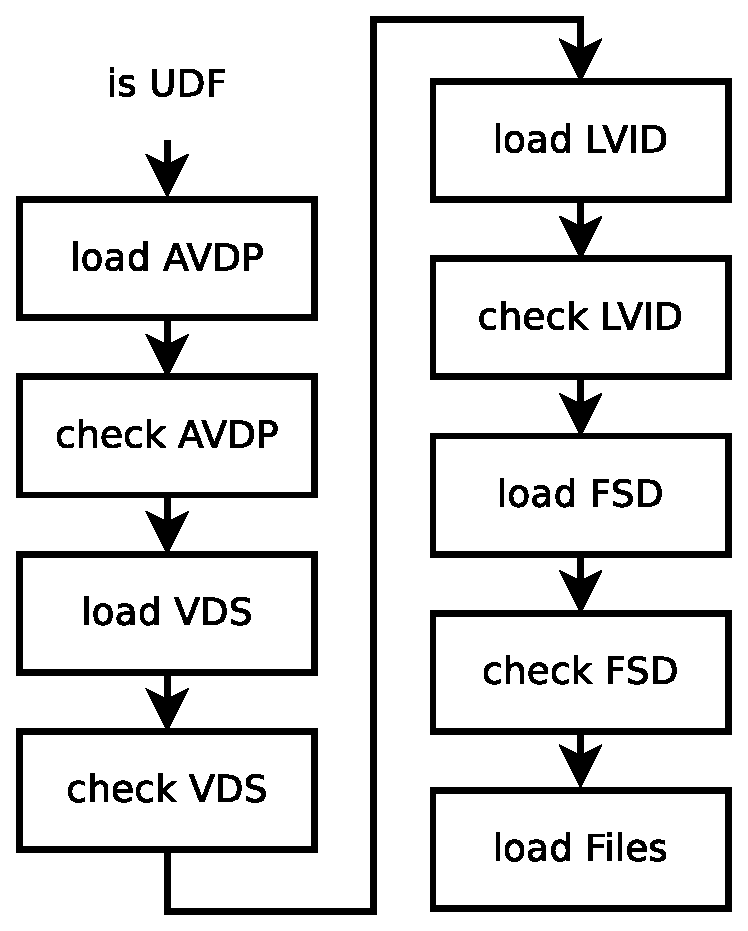
\includegraphics[scale=0.4]{obrazky/steps1.eps}
    \caption{Zjednodušený alogoritmus činnosti programu}
    \label{fig:steps1}
\end{figure}

\subsection{Výstup a ovládání nástroje}
Nástroj \texttt{udffsck} je navržen po vzoru ostatních nástrojů z rodiny \texttt{fsck}. Tomu bude odpovídat i jeho ovládání a výstup.\\
Vstupy různých \texttt{fsck} nástrojů se liší podle jednotlivých souborových systémů, ale kvůli zapouzdřitelnosti musí dodržovat návratové hodnoty pro různé druhy chyb. Jedná se o tyto hodnoty:
\begin{itemize}
    \item 0 - Bez chyb 
    \item 1 - Opraveny chyby na souborovém systému
    \item 2 - Opraveny chyby na souborovém systému, doporučený reboot 
    \item 4 - Chyby souborového systému zůstaly neopraveny
    \item 8 - Chyba programu
    \item 16 - Chybné vstupní parametry
    \item 32 - Kontrola byla přerušena na základě uživatelského požadavku
    \item 128 - Chyba sdílené knihovny
\end{itemize}
Návratová hodnota může být i součet těchto hodnot pokud nastalo více chyb zároveň.\\
Má implementace v tuto chvíli nerespektuje tyto hodnoty z důvodů vývoje a vrací různé chybové kódy podle místa kde program skončil. Toto chování bude nahrazeno lepšími výpisy do standardního výstupu a chybového výstupu.\\
Jedná se o terminálový program bez jakéhokoli grafického uživatelského rozhraní nebo i textového uživatelského rozhraní. Běh programu je možné ovlivnit pouze jeho vstupními parametry, které jsou dodány při jeho spuštění spolu s médiem ke kontrole. Jeho výstupy jsou směrovány na standardní výstup \texttt{stdout} a chybový výstup \texttt{stderr}. V tuto chvíli není výstup programu sjednocený do uživatelsky přívětivé podoby ale spíše pro vývojáře, protože se vypisuje vysoké množství ladicích a informativních údajů.\\
Program v tuto chvíli vyžaduje k běhu informaci o velikosti sektoru média a médium samotné. Volání programu může vypadat například takto:\\ 
\centerline{\texttt{./udffsck -b 2048 medium.img}}\\
První je samotný program, poté následuje povinný parametr \texttt{-b} následovaný velikostí fyzického sektoru. Mezera mezi paramtrem a hodnotou není povinná. Posledním paramterem je samotné kontrolované médium. Jemu nepředchází žádný identifikátor.\\
Ukázkový výstup programu je v příloze \ref{lst:bs512} včetně komentáře jednotlivých částí výstupu. 

\subsection{Načtení média a jeho příprava na zpracování}
Kontrolované médium je otevřeno pomocí standardního systémového volání \texttt{open}, v tuto chvíli pouze pro čtení. Takto otevřené médium je vzápětí pomocí funkce \texttt{mmap} namapováno do paměti aby se dalo s médiem pracovat jako s bytovým polem a ne jako se souborem. Posléze je soubor uzavřen, protože ve chvíli, kdy byl úspěšně namapován byla jeho reference zkopírována a začala být udržována operačním systémem, který ji zruší až nebudou žadné části souboru namapované do paměti (viz \cite{posix-mmap}). 

\subsection{Algoritmus načtení AVDP}
AVDP je klíčovou částí UDF, protože určuje výchozí bod pro čtení souborového systému. Jak je uvedeno v kapitole \ref{sec:avdp}, UDF rozlišuje čtyři možná umístění AVDP, přičemž přítomny mohou být až tři na médiu.\\
Jejich načítání pro potřeby další práce se souborovým systém lze popsat algoritmem na obrázku \ref{fig:avdp}. Alogoritmus prochází možné lokace AVDP dokud neuspěje nebo nedojdou možnosti. Pro potřeby kontroly a opravy média je třeba po nalezení alespoň jednoho správného AVDP ostatní podle něj opravit.
\begin{figure}[ht] 
    \centering
    %\resizebox{0.5\textwidth}{!}{\input{obrazky/avdp.tex}}}
    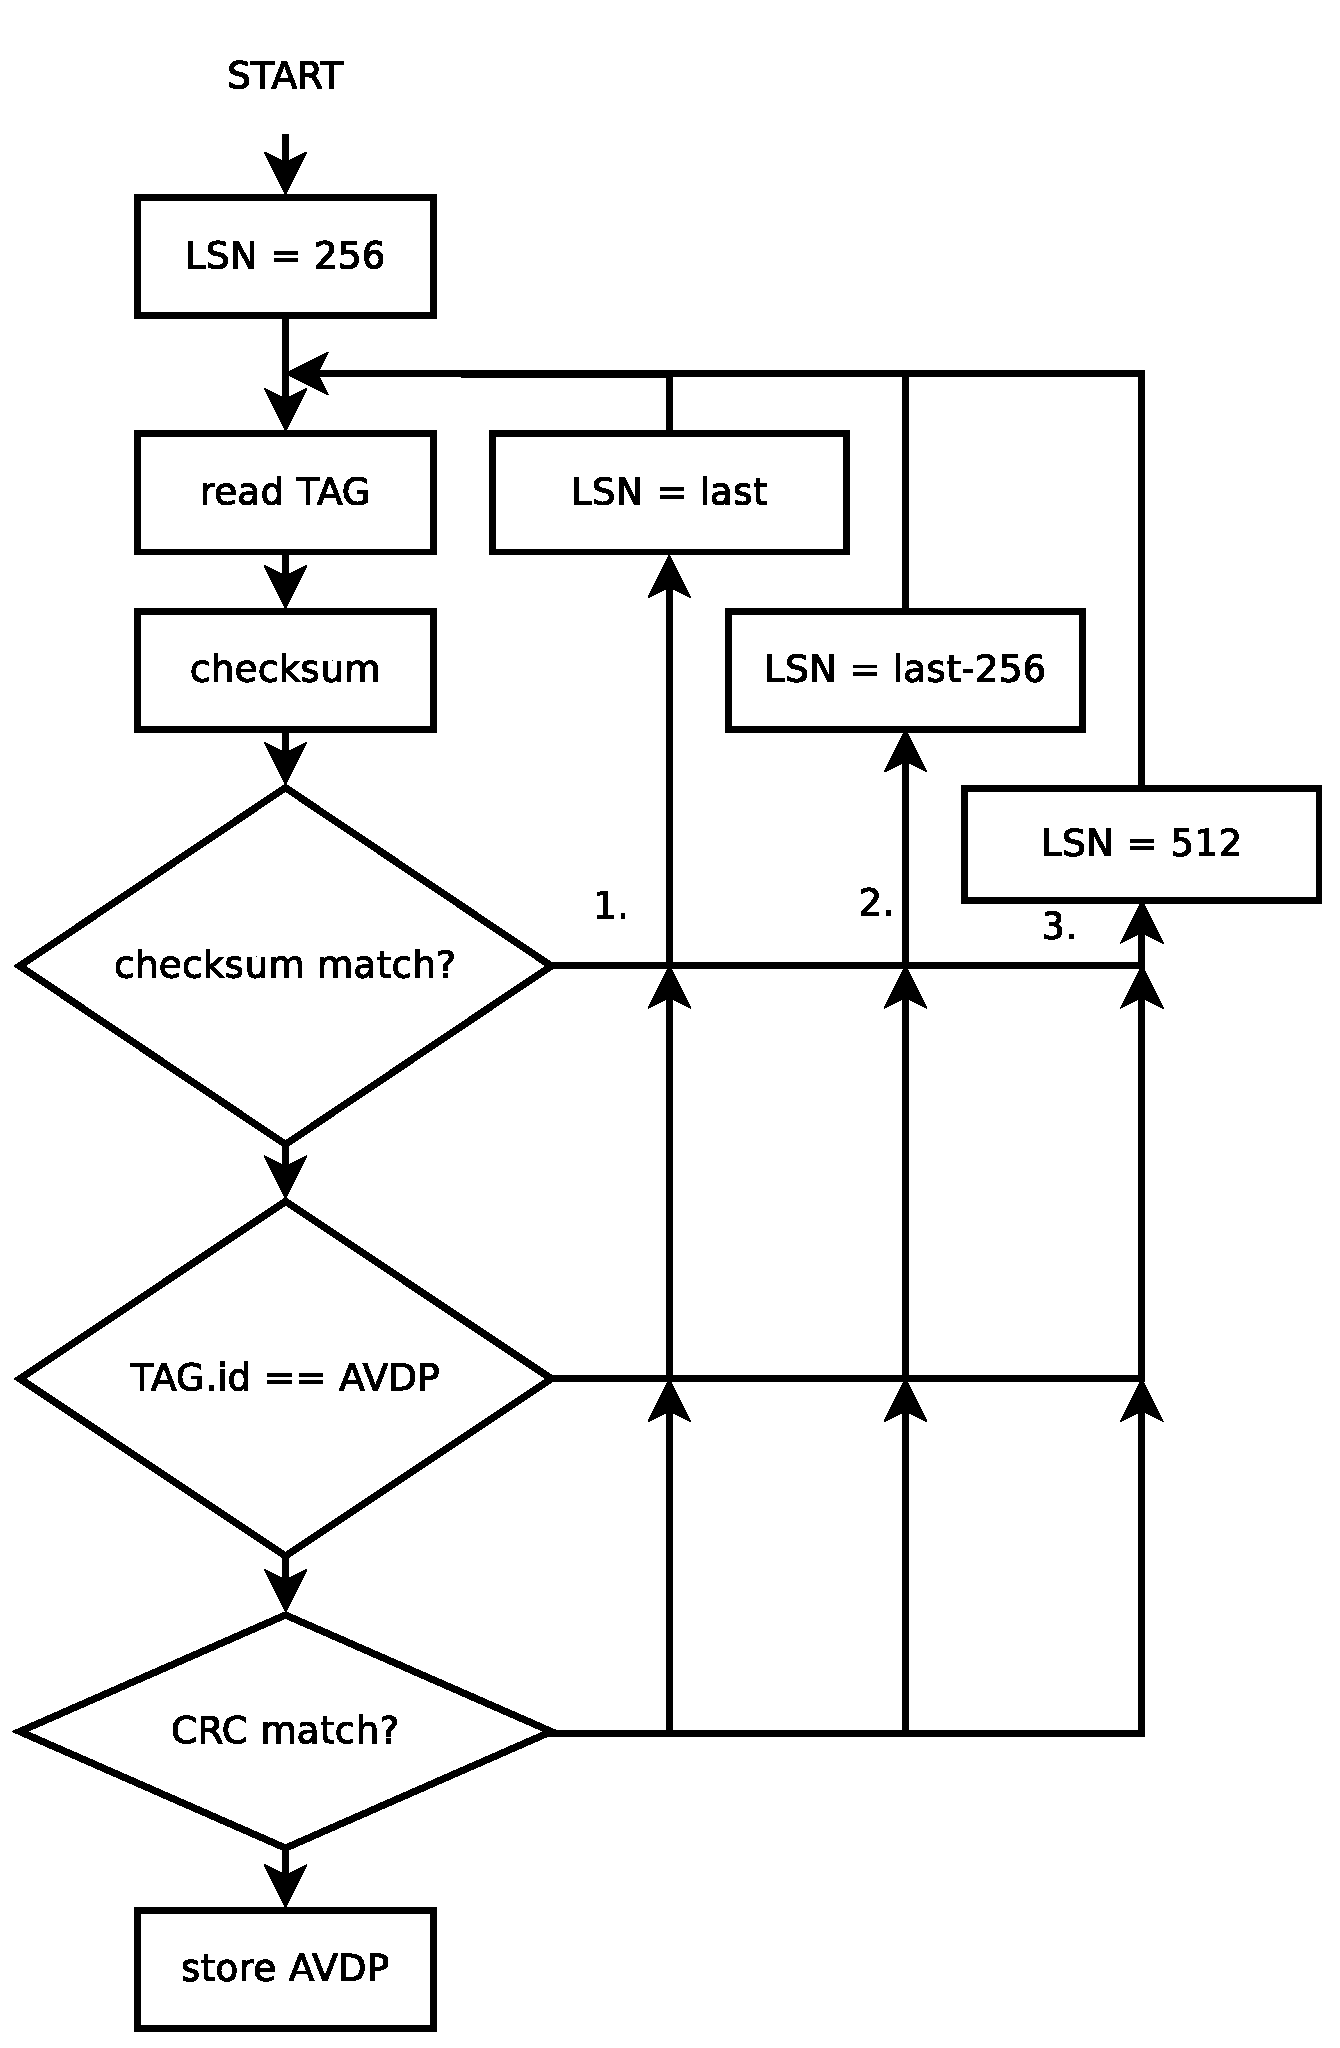
\includegraphics[scale=0.4]{obrazky/avdp.eps}
    \caption{Zjednodušený algoritumus načtení AVDP}
    \label{fig:avdp}
\end{figure}

\subsection{Algoritmus čtení souborů}
Obnova uživatelských dat je klíčová část programu. Bez ní nemá tento nástroj význam. Vzhledem k faktu, že UDF neimplementuje ochranné algoritmy na data samotná ale jen na metadata, není bohužel možné poškozená data ani detekovat, ani obnovit. Je možné se pokusit zrekonstruovat adresářovou strukturu a místo, kde by data měla být.\\
Algoritmus načtení adresářové strkutury je zachycen na obrázku \ref{fig:files}. Tento algoritmus začíná po úspěšném načtení FSD, odkud je získána pozice FE kořenového adresáře (proto algoritmus začíná čtením FE). Pokud je toto úspěšné, pokračuje se k čtení FID a takto se postupně projde celou strkturou.\\
Místa na obrázku označnená jako \textit{ERROR} značí místa, kde došlo k chybě některého z kontrolních mechanismů a bylo by nutné přistoupit k obnově. 
\begin{figure}[ht] 
    \centering
    %\resizebox{0.5\textwidth}{!}{\input{obrazky/avdp.tex}}}
    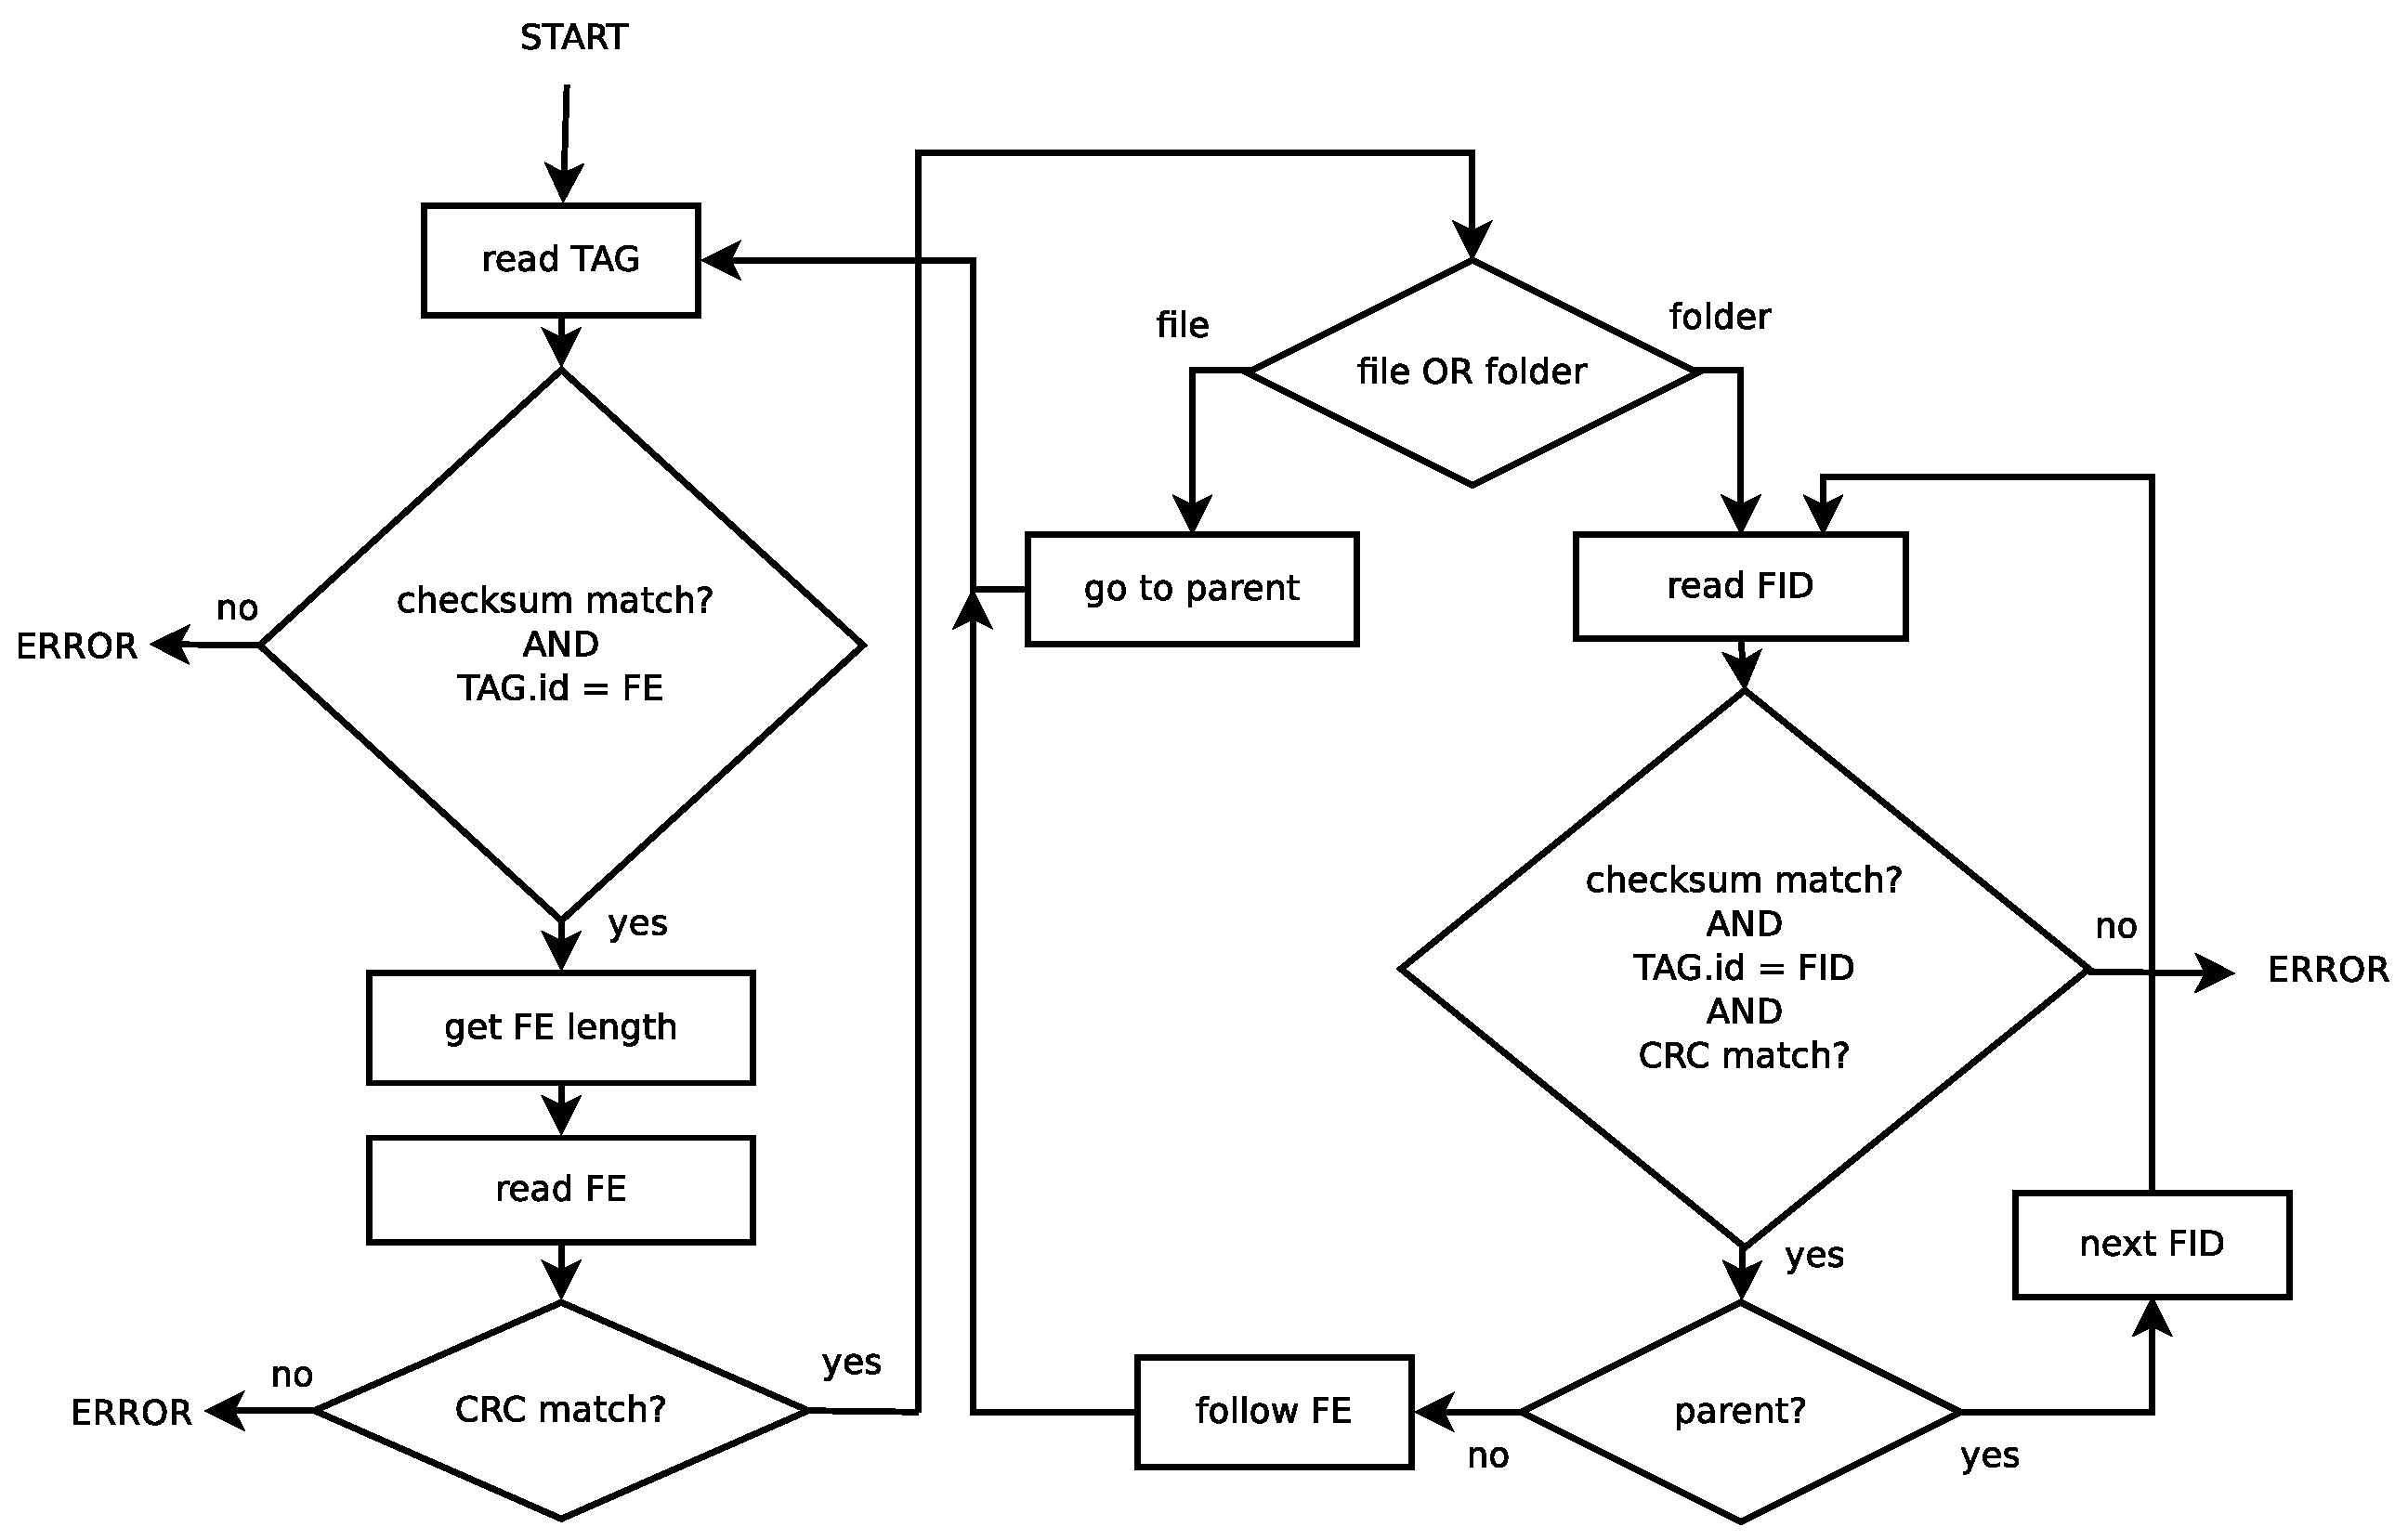
\includegraphics[scale=0.36]{obrazky/files.eps}
    \caption{Algoritmus načítání souborů}
    \label{fig:files}
\end{figure}

\subsection{Detekce chyb na médiu}
Detekce chyb na médiu je v tuto chvíli implementována pouze na úrovni porovnání kontroloních součtů a CRC.\\
Kontrolní součty jsou implementovány mou funkcí\\
\centerline{\texttt{\detokenize{uint8_t calculate_checksum(descTag tag)}}}\\
v souboru \texttt{udffsck.c}. Tato funkce pouze počítá checksum nad zadaným tagem a výsledek vrací. Proto je zapouzdřena do funkce\\
\centerline{\texttt{\detokenize{int checksum(descTag tag)}}}\\
která přidává porovnání se checksum v tagu. Takto fukce vrací 0 při rozdílu a nenulovou hodnotu při shodě.\\
CRC je počítáno funkcí sdílené knihovny, která je součástí balíku. Ta byla opět zapouzdřena funkcí\\
\centerline{\texttt{\detokenize{int crc(void * desc, uint16_t size)}}}\\
aby vracela tentokrát 0 při neshodě a nenulovou hodnotu při shodě. Oproti funkci pro výpočet kontrolního součtu je třeba funkci pro výpočet CRC dodat i délku. Důvodem je, že \textit{DescriptorTag} má fixní délku a tu lze zjistit ze struktury, která jej popisuje pomocí funkce \texttt{sizeof}. Deskriptory ovšem tuto vlastnost nemají. Jsou deskriptory, které mají délku fixní, ale část má délku proměnnou podle dat, která nesou (například délka struktury \textit{File Entry} se závislá na tom jestli se jedná o soubor nebo adresář a v případě adresáře ještě kolik dalších deskriptorů je uvnitř.)

